\documentclass{article}
\usepackage{graphicx} % Required for inserting images
\usepackage{amsmath}
\usepackage[margin=1in]{geometry}
\usepackage{listings}
\usepackage{array}

%Document
\begin{document}

\vspace*{\fill}   % Centers the title vertically on the page

\begin{center}
    {\LARGE Engineering Requirements Document \\}   % Title in Large font
    \vspace{1cm}         % Space between title and author name
    {\large Lucas Butler \\}  % Author name in a smaller font than the title
    \vspace{1cm}         % Space between author name and date
    {\large \today}      % Today's date in a smaller font
\end{center}

\vspace*{\fill}   % Fill the rest of the page

\newpage

\section{Product Definition}

\subsection{Summary}
\quad In the United States, Cardiac disease produces a significant number of casualties, nearly 700,000 deaths a year \cite{cdc}. Currently, anomalies such as irregular heart rhythms (arrhythmia) and blood flow blockages (myocardial infarction) are monitored through the collection and classification of Electrocardiogram signals. These signals are typically collected in a clinical setting, through electrodes and wires under the supervision of Doctors and Nurses and take a significant amount of time to be sifted through and classified. The current state of this pipeline requires significant effort from medical professionals, yet yields low volumes of patients receiving the care they need, compared to the demand. 

\subsection{Identification}
In order to alleviate the bottlenecks created by the current system, significant infrastructural improvements must be achieved. To make access of ECG signal acquisition more ubiquitous, Internet of Things, Cloud, and Machine learning technologies will need to extend upon tradition Digital Signal Processing algorithms and cutting edge computer hardware.

At the edge, a power-efficient ECG sensor node capable of long range data communication can be utilized to collect ECG data. The use of wireless communication will erase the need to enter a clinical setting and make the classification technology available to more patients. It will also eliminate the need for wires and stand-alone monitoring systems, which will reduce tripping hazards in operation settings and reduce asset maintenance costs. 

With wireless data collection and communication, employing a cloud-based approach to monitoring signals will now be feasible. This approach will utilize communication across the web, transmitting data to a centralized database. Data stored would be accessible through a web interface, releasing constraints over location  and providing a comprehensive over view for all patients in a one stop shop. An optimal approach to development would be in the form of a deployable cloud container that scales with the number of requests for service. This cloud container could be deployed within the hospital or clinical network for internal usage or by a business on a local server for servicing individual patient requests outside of a clinical setting.

To assist in the prioritization and classification of cases, Machine Learning technologies, such as Convolutional Neural Networks, can operate on the data stored in the cloud server. These neural networks can identify target patterns in signals and predict anomalies with high accuracy. 

\subsection{Users}
This project contributes to society by improving the efficiency of triage within the health care system, in addition to making cardiac telemetry more accessible. A versatile ECG signal classification system will serve a wide variety of health professionals, patients at-risk, and the general population.

This technology will be heavily utilized by hospitals and clinics. Centralized monitoring will enable a more informed view for medical professionals to utilize in their decision making. Automating the collection and detection of anomalies will improve prioritization of patients and provide more opportunity to prevent failure, significantly contributing to the health care effort. Researchers will benefit from additional medical data when discovering root causes and fine tuning their assessment policies. Introducing this streamlined approach will empower medical professionals to excel in their responsibilities.

Patients will greatly benefit from ubiquitous ECG classification. Those at-risk are typically worried about abnormalities and feel tied to hospitals or clinics for consistent updates. Unrestricted cardiovascular monitoring will relieve this stress by facilitating patient autonomy and fostering a deeper engagement with more enjoyable daily tasks. With improved insight, those at-risk will be able to self-assess the challenges they face during various activities, introducing a drastic improvement in the average quality of life. 

Everyone, including those who are not considered at-risk or health professionals, will benefit. Providing deeper insights into cardiovascular health will allow individuals to make better decisions about their eating, exercising and sleeping habits. Athletes and fitness enthusiasts will utilize this information to prep for important matches and improve training regiments. Post-op surgery patients will benefit from smoother recovery, and the Elderly will rest assured that they are in good health.

\subsection{Interfaces}
User Profile: Each patient will be prompted to generate a unique profile. The profiles will employ multi-factor authentication through text message, phone call, or email verification to increase the security of sensitive medical data. Through this unique profile, patients will be able to connect their with medical providers, allowing medical professionals to read and analyze their data. This feature will be enabled at the discretion of the user and can be revoked without external consent, giving users full control over their data.

Data Presentation: A dashboard for the centralized database will provide a comprehensive overview of heart health. Graphs with information regarding periods of irregular heart beat, heightened activity and exercise patterns are all relevant and can be utilized to assess risks and habits of patients. In addition, medical professionals will have the option to view multiple patients data in realtime, giving them greater control over the nursing station.

Sensor Node: Wireless sensor nodes should be easily operable by patients and practitioners. The connectivity protocol should be simple; turn on the sensor and press a button to initiate the connection protocol. An LED indicator on the node will indicate the state of connection, communication, and indicate if the battery is getting low.

\newcolumntype{M}[1]{>{\centering\arraybackslash}p{#1}}
\subsection{User Requirements}
\begin{table}[h]
    \centering
    \begin{tabular}{|M{0.3cm}|p{4cm}|p{5cm}|}
        \hline
        \# & Requirement & Description \\
        \hline
        1 & Email & Access to an email account. Important for generating a user profile. \\
        \hline
        2 & Phone Number (optional) & Account verification and security. \\
        \hline
        3 & Internet Access & Access to services. \\
        \hline
        4 & Electrical Outlet & Access to power is required for charging the sensor node. \\
        \hline
        5 & Computer/Mobile Device with Browser & All services are accessed through a web portal. A device with a web browser is essential. \\ 
        \hline
        6 & Knowledge about Heart Health & A basic understanding of heart beat and the cardiovascular system is important to get value out of the product. \\
        \hline
        7 & Sensor Node & A device capable of collecting ECG signals and transmitting them via wireless protocol. \\
        \hline
    \end{tabular}
    \caption{User Requirements}
    \label{tab:example}
\end{table}

\newpage
\subsection{Customer Needs}

\begin{table}[h]
    \centering
    \begin{tabular}{|M{0.3cm}|p{1.2cm}|p{4cm}|p{5cm}|}
        \hline
        \# & Need \# &Requirement & Description \\
        \hline
        1 & 1a & Secure data transmission & All data transmission should be encrypted to ensure privacy of user information. \\
        \hline
        2 & 2a & Accurate Classification & Captured signals should be high quality. Classifications of signals should be highly accurate ensuring customer confidence.  \\
        \hline
        3 &  & Real Time Updates & Over system latency should low and give real-time updates on the current state of health. \\
        \hline
        4 & & Notifications & A robust notification system that updates both patients and medical professionals when an emergency is occurring.\\
        \hline
        5 & & Help Desk Service & A 24/7 assistance service that helps users with setting up the system, troubleshooting issues, and for providing additional information to enable thorough extraction of product value. \\ 
        \hline
        6 & & Cloud Storage & Centralized, secure storage of user data to enable ease of access from any device at any time. \\
        \hline
        7 & & Simple, Intuitive UI/UX & The user experience design should reduce as much complexity as possible, giving users easy access to the features they need, and hide away the unhelpful information. \\
        \hline
    \end{tabular}
    \caption{Customer Requirements}
\end{table}

\newpage
\section{Project Definition}

\subsection{Summary}
The focus of implementation will be on the design of the sensor node, more specifically, the data path. This design will include the signal capture and preprocessing circuitry, digital filtering, encryption, packaging and sending of the signal data through a wireless protocol. This will involve selecting the appropriate hardware, programming the boot-up, algorithms, and operating system used in the node, and if time permits, designing power circuitry.

\subsection{Constraints and Limitations}
Time constraints are a major limitation as researching, designing and developing this project in one semester will allow little room for revision. Technical complexity when implementing the electronics and algorithms will make it difficult to produce an accurate and reliable system. Budget limitations will limit the options for part selection, providing additional quality assurance challenges. Packaging the sensor into a discrete and power efficient form factor will be technically demanding and require significant research and iteration, which time will not permit. Abiding to all the regulations specified by the FDA and HIPAA will also be a challenge due to the shear quantity and limited time to get familiar. Testing and validation of the system will require careful consideration and is limited by the equipment available in the labs at Chico State University and experience.

\subsection{Assumptions and Dependencies}
Signal characteristics of ECG are as follows: 0.05-100 Hz, input voltage of 0.5-5.0 mV \cite{adialogue} from the electrode. The device will be used within a 50 meter radius of the signal receiving machine. Various forms of noise such as electrode contact (0-20 Hz), various bodily signals (0.13-3 Hz), and motion artifacts (0-20 Hz) will be present in the signal \cite{ecgfiltering}. Power line noise in the range of 50-60 Hz can be neglected due to battery operation. Using the Nyquist theorem as a baseline, the signal will be sampled at 500 Hz to put us far above 200 Hz, produced by the equation $S = 2 * f$. Targeted power consumption of the system will be around 500 mW to provide buffer over the implementation done by Yang et. all \cite{yang} of a wireless EMG sensor node using Bluetooth LE protocol and analog digital filtration which consumed 343 mW. HIPAA imposes strict regulations on Personal Health Information and suggests using 128-bit AES as the standard encryption protocol F\cite{sprinto}. The system will be design in such a way that the electrodes are removable and replaceable. 

\newpage
\subsection{Architecture}

\begin{figure}[h]
    \centering
    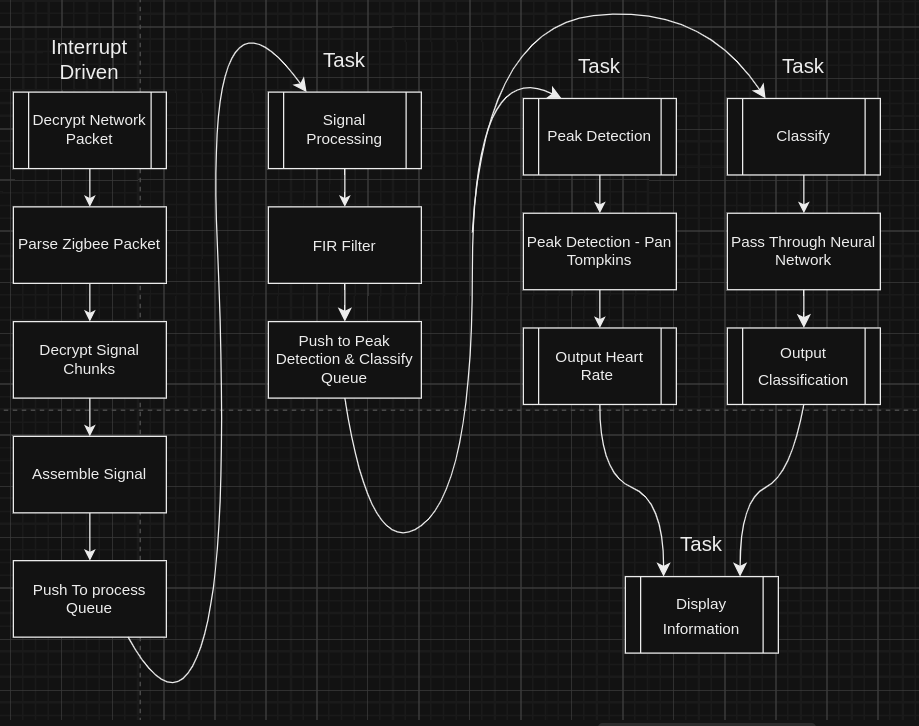
\includegraphics[width=4in, height=4in]{flow1.png}
    \caption{Software flowcharts part 1.}
\end{figure}

\begin{figure}[h]
    \centering
    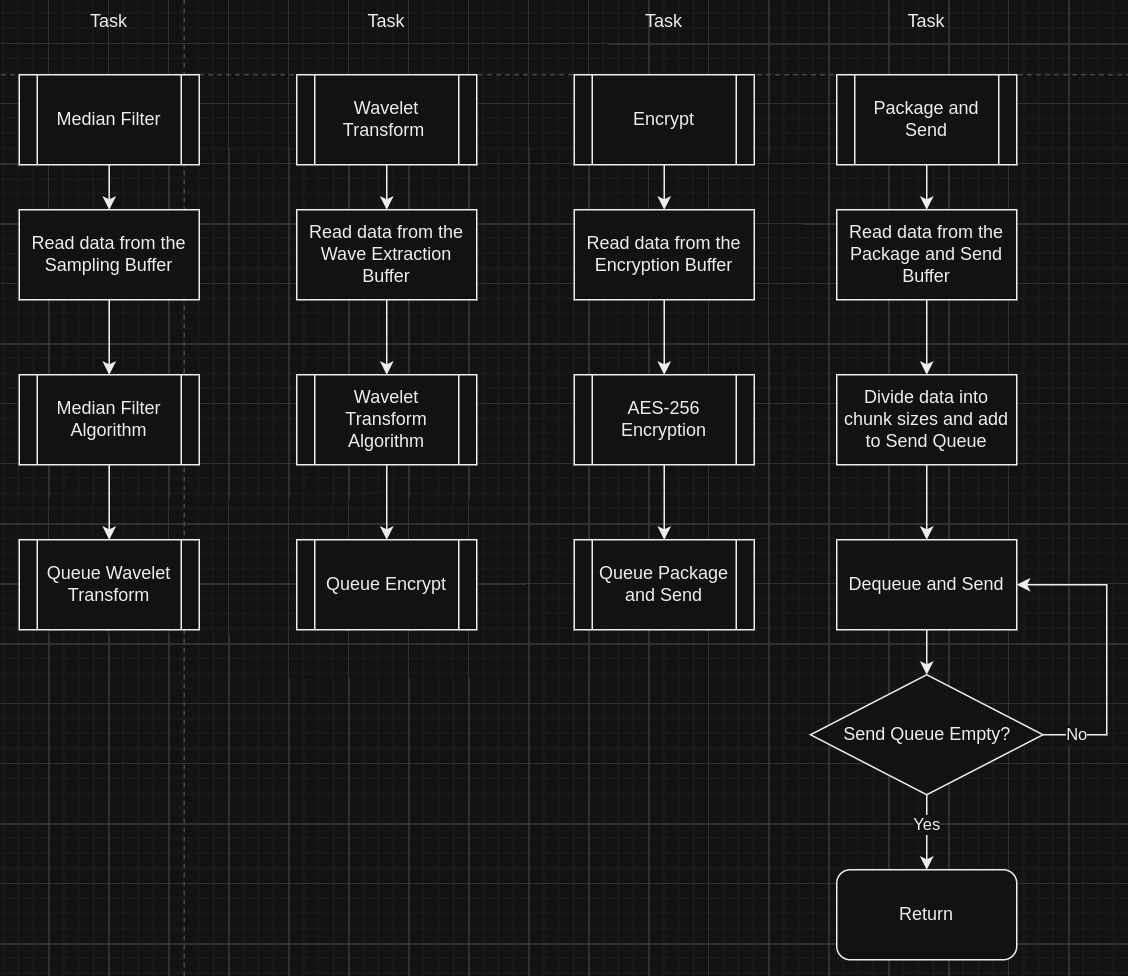
\includegraphics[width=4in, height=3.5in]{flow2.png}
    \caption{Software flowcharts part 2.}
\end{figure}

\newpage
\subsection{Design Alternatives}
Signal acquisition can be carried out in a variety of ways, each with considerations of power efficiency, signal integrity, complexity and flexibility. One approach that was heavily considered was utilizing an array of op-amps for signal amplification and filtering, then sampling the signal using the microcontroller's built in ADC. While this route would enable design for optimum power efficiency and yields the best signal quality, using this type of hardware is generally less flexible when making adjustments to the system is needed to fine-tune performance. In the event that the behavior of the circuit does not reflect the results of the simulation, new values of resistors and capacitors must be selected, purchased and physically implemented. The time constraint forces prioritization of a more flexible system, making a programmable ADC and algorithmic digital filtering more desirable.  Using a programmable ADC and digital filtering algorithms, we can change gain and filtering characteristics via software parameters, which will allow for quick turnover when making adjustments. \par

Wireless communication protocol selection is a critical design choice for this project. There are various design requirements to identify when choosing a protocol. First, the receiving station must be able to receive signals from multiple sensors at once. Second, the communication protocol must be low power in order to maximize the battery life of the sensor. Third, the data rate needs to support transmitting a minimum of 500 samples of 2-byte data a second from the signal acquisition system, yielding the minimum rate of 8 Kbps. Wi-Fi and Bluetooth communication protocols were identified as alternatives instead of Zigbee, but were later found to have issues satisfying the requirements. Wi-Fi is overpowered when it comes to data transmission as normal rates for 802.11b are in the Mbps range \cite{cisco}, when we only require Kbps transmission. Wi-Fi transmission is relatively power hungry due to this. Another option that was considered is Bluetooth Low Energy (BLE). BLE 4.0 data rates are much more comparable to Zigbee, in the range 125 Kbps - 2 Mbps \cite{nordic}, and is designed for lower energy consumption. The main difference between BLE and Zigbee is the network topology. BLE adopts a Master-Slave topology and limits the master to 8 devices for communication \cite{ehub}. On the contrary, Zigbee uses a mesh network topology which allows for large-scale networks on the order of 65000 cell nodes. A major benefit of using Zigbee is that the mesh network topology allows for extended communication ranges by enabling data to hop between devices to reach its destination, extending range to 291 meters, whereas BLE can transmit a mere 77 meters. For designing scalable sensor node systems, Zigbee is the best choice. 

\subsection{Specifications}
\begin{table}[h]
    \centering
    \begin{tabular}{|M{0.3cm}|p{1.2cm}|p{4cm}|p{5cm}|}
        \hline
        \# & Need \# & Requirement & Ideal Value \\
        \hline
        1 & & Target Frequency Band & 0-50 Hz \\
        \hline
        2 &  & Input Signal Voltage \cite{adialogue} & 0.5-5.0 mV \\ 
        \hline
        3 &  & Signal Sampling Rate & 500 Hz \\
        \hline
        4 &  & Data Encryption & AES-256  \\
        \hline
        5 &  & Wireless Connectivity & Zigbee PRO\\
        \hline
        6 &  & Wireless Data Transmission & 8 Kbps \\
        \hline
        7 &  & Transmission Distance & 50 meters for a signal node \\
        \hline
        8 &  & Latency & 0.5 seconds from when signal data for the current time frame has been captured to when it arrives at the host device. \\
        \hline
        9 &  & Signal Capture Window 0& 3 seconds of signal capture for one data batch. \\ 
        \hline
        10 &  & Removable Electrode & Yes \\ 
        \hline
        11 &  & Power Consumption \cite{adialogue} & 500 mW or less \\ 
        \hline
    \end{tabular}
    \caption{Customer Requirements}
\end{table}


\subsection{Project Schedule}
\begin{figure}[h]
    \centering
    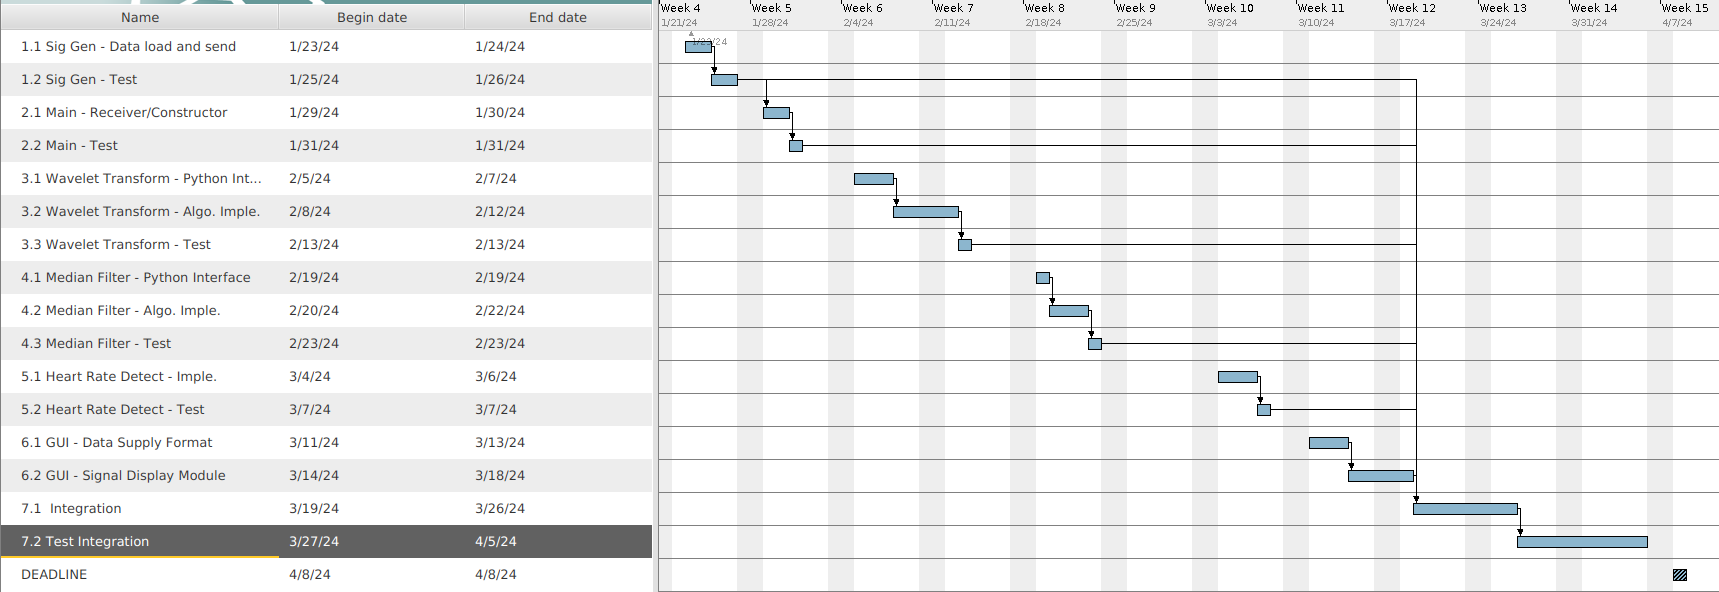
\includegraphics[width=6in, height=2in]{Gantt.png}
    \caption{Gannt chart of the project.}
\end{figure}

\newpage
\subsection{Prototype Costs}

\begin{figure}[h]
    \centering
    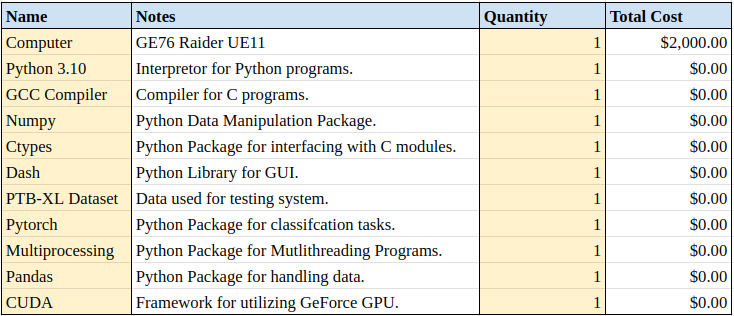
\includegraphics[width=5in, height=2in]{BOM.png}
    \caption{Bill of materials for project.}
\end{figure}

\section{References and Standards}
\begin{thebibliography}{9}
    \bibitem{cdc}
    Centers for Disease Control and Prevention, ``Heart Disease Facts.'' Available: https://www.cdc.gov/heartdisease/facts.htm.
    
    \bibitem{acc}
    American College of Cardiology, ``Chronic Coronary Disease Guidelines (2023).'' Available: https://www.acc.org/Guidelines/Hubs/Chronic-Coronary-Disease.
    
    \bibitem{cisco}
    Cisco, `RF Design Considerations,' Cisco Systems, Inc. [Online]. Available: https://www.cisco.com/en/US/docs/solutions/Enterprise/Mobility/
    emob30dg/RFDesign.html. [Accessed: Nov. 20, 2023].
    
    \bibitem{nordic}
    `The complete guide to Bluetooth Low Energy', Nordic Semiconductor. [Online]. Available: https://response.nordicsemi.com/the-complete-guide-to-bluetooth-low-energy. [Accessed: Nov. 20, 2023].
    
    \bibitem{ehub}
    `Zigbee Vs Bluetooth,' ElectronicsHub. [Online]. Available: https://www.electronicshub.org/zigbee-vs-bluetooth/. [Accessed: Nov. 20, 2023].
    
    \bibitem{adialogue}
    `ECG Front-End Design is Simplified with MicroConverter,' Analog Dialogue. [Online]. Available: https://www.analog.com/en/analog-dialogue/articles/ecg-front-end-design-simplified.
    
    \bibitem{ecgfiltering}
    S. Nayak, M. K. Soni, and D. Bansal, ``Filtering Techniques for ECG Signal Processing,'' in International Journal of Research in Engineering \& Applied Sciences, vol. 2, no. 2, pp. 671, Feb. 2012. [Online]. Available: http://www.euroasiapub.org. [Accessed: Nov. 20, 2023].
    
    \bibitem{yang}
    Y. -H. Yang, S. -J. Ruan, P. -C. Chen, Y. -T. Liu, and Y. -H. Hsueh, ``A Low-Cost Wireless Multichannel Surface EMG Acquisition System,'' in IEEE Consumer Electronics Magazine, vol. 9, no. 5, pp. 14-19, 1 Sept. 2020, doi: 10.1109/MCE.2020.2986792.
    
    \bibitem{sprinto}
    Sprinto, ``List of HIPAA Encryption Requirements,'' Sprinto. [Online]. Available: https://www.sprinto.com/compliance/hipaa-encryption-requirements/.
\end{thebibliography}
    
\section{Appendix}
\end{document}